\documentclass[conference]{IEEEtran}
\IEEEoverridecommandlockouts
% The preceding line is only needed to identify funding in the first footnote. If that is unneeded, please comment it out.
\usepackage{cite}
\usepackage{amsmath,amssymb,amsfonts}
\usepackage{algorithmic}
\usepackage{graphicx}
\usepackage{textcomp}
\usepackage{hyperref}
\usepackage{xcolor}
\usepackage{listings}
\usepackage{markdown}
\def\BibTeX{{\rm B\kern-.05em{\sc i\kern-.025em b}\kern-.08em
    T\kern-.1667em\lower.7ex\hbox{E}\kern-.125emX}}
\begin{document}

\title{5. Radio payload}

\author{\IEEEauthorblockN{Jakub Šmíd}
\IEEEauthorblockA{\textit{Course: Space Engineering \the\year} \\
\textit{Czech Technical University in Prague}\\
Technicka 2, Prague, Czech Republic \\
smidjak3@fel.cvut.cz}
\and
\IEEEauthorblockN{Josef Vágner}
\IEEEauthorblockA{\textit{Course: Space Engineering \the\year} \\
\textit{Czech Technical University in Prague}\\
Technicka 2, Prague, Czech Republic \\
vagnejos@fel.cvut.cz}
\and
\IEEEauthorblockN{Ing. Ondřej Nentvich, Ph.D.}
\IEEEauthorblockA{\textit{Course: Space Engineering \the\year} \\
\textit{Czech Technical University in Prague}\\
Technicka 2, Prague, Czech Republic \\
ondrej.nentvich@cvut.cz }
}

\maketitle

\begin{abstract}
This report reviews what the communication protocols are composed of. It describes how Cubesat Space Protocol and Bluetooth Low Energy work. The practical part of this project deals with communication between nRF52 on the server side and the Python script on the client side.
\end{abstract}


\section{Assignment}
Develop a program for the Radio payload that can handle communication for the CubeSat.
\begin{itemize}
\item Propose communication between Radio payload (nRF52832) and Ground station (PC in this case) in S-band.
\item The communication is based on CSP protocol.
\item Establish communication between the radio part (nRF52832) and the microcontroller, which will handle communication with the rest of the CubeSat (STM32F413).
\item Optionally: Develop a program (in Python) for the ground station to manage communication with the CubeSat.
\item Selected MCUs are STM32F413 and nRF52832.
\end{itemize}

\section{Introduction}
This project aims to review space communication protocols, especially the Cubesat Space Protocol. Also, the goal is to get working communication between the radio board of the school demo Cubsat (CVUT-SAT\cite{CVUT-SAT} shown in the figure \ref{cvut-sat}) and a ground station (PC).

\begin{figure}[htbp]
    \centerline{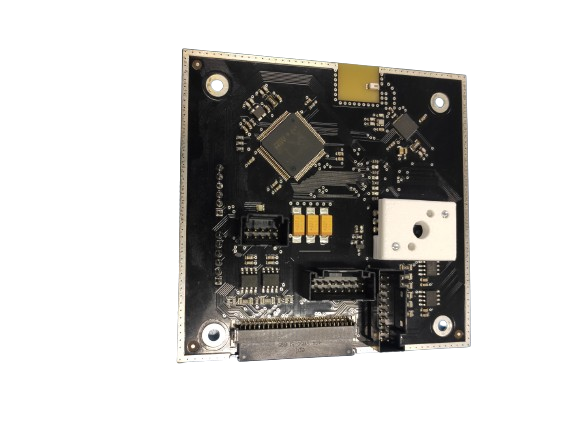
\includegraphics[scale=0.4]{images/radio-pcb}}
    \caption{Radio board of CVUT-SAT}
    \label{cvut-sat}
\end{figure}

It is composed of STM32F413, which can serve as a backup onboard computer. This processor is connected via CAN bus with another chip, nRF52832, which is capable of communication via Bluetooth Low Energy. The nRF processor is the main subject of our interest because it is a gateway of communication between the Ground station and the CubeSat.

\begin{figure}[htbp]
\centerline{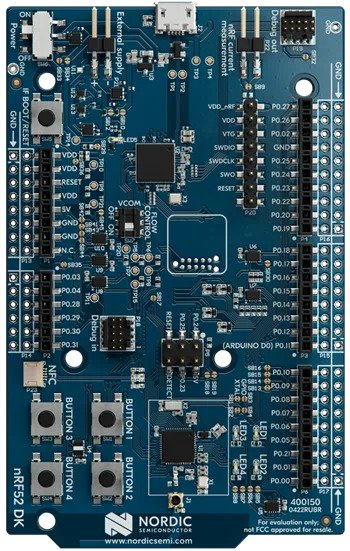
\includegraphics[scale=0.4]{images/nRF52-DK}}
\caption{nRF52 DK - Bluetooth Low Energy and Bluetooth mesh development kit for the nRF52810 and nRF52832 SoCs\cite{nrf-dk-shop}}
\label{nrfDK}
\end{figure}

The nRF52832 needs a programmer, so we have been given nRF52 DK \cite{nrf-dk-shop} (development kit shown in the figure \ref{nrfDK}). The major part of this project was developed using this DK. The development kit contains a debugger and also nRF52832. A debugger can also be used to emulate different nRF52 processors. The kit has four buttons and four LEDs, so we can easily interact with the hardware.

The debugger on the development kit can be connected to the CubeSat radio board using a particular programming jumper. It is possible to program/debug the nRF chip on the board. STM32 processors commonly have a proprietary bootloader, which adds the possibility of downloading new firmware directly without using a programmer. On the other hand, you cannot debug the STM with this setup.

At the beginning of this report, we will describe the ISO/OSI model, which is commonly known and used for describing communication protocols. Then, we will introduce some communication protocols and describe the Cubesat Space Protocol, which we used in this project. Then, we will describe Bluetooth. At the end, we will describe the laboratory part of our project. It means we propose our solution for the problem and describe the provided code for the nRF and the Ground station.

\section{OSI model}
The OSI model stands for the Open Systems Interconnection model, a foundational framework for understanding and designing communication protocols. It provides a systematic approach to conceptualizing and implementing network communication, ensuring interoperability between different systems. In 1983, OSI was adopted by the International Organization for Standardization (ISO) as ISO 7498, with the current version being ISO/IEC 7498-1:1994\cite{AWS-Amazon}. Since then, it has been adopted by all major computer and telecommunication companies. It was the first standard model for network communication. \cite{impreva-osi}

Because there are many incompatible machine technologies, the standard concept allows us to agree on how two computer systems could exchange data; it helps visualize how digital communication operates. So, before we dive deep into the space communication protocols, we describe this OSI model. The OSI model would be a good reference point. Besides better understanding the space protocols, the OSI model also aids in developing and evaluating protocols.

The OSI model comprises seven abstract layers in the figure \ref{osi}. Each layer has a specific purpose and functionality to perform. Each layer is independent and interacts directly with two other layers - layer above and below. However, all layers work collaboratively and describe how the user/application data are transmitted. Using these layers allows for a more systematic approach to networking. Instead of having a huge communication system, we can split it into these layers, each performing a specialized transmission function. \cite{geeks-osi}

\begin{figure}[htbp]
    \centerline{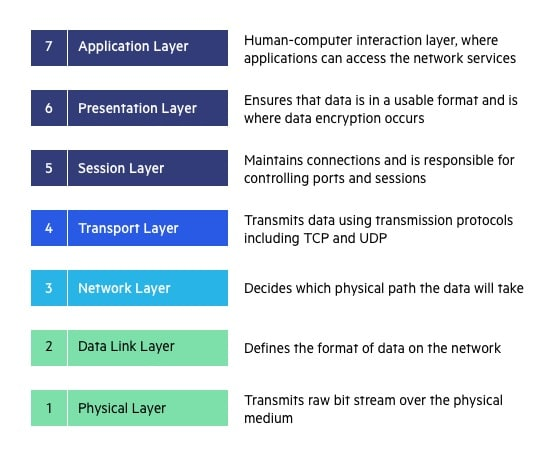
\includegraphics[width=\linewidth]{images/OSI-7-layers}}
    \caption{Layers of the OSI model\cite{impreva-osi}}
    \label{osi}
\end{figure}

The process of sending data using OSI is as follows: first, the sender application has to pass the data to the application layer, which passes them down to the next lower layer. Then, each layer adds its headers before passing it on. The data communication moves down the layers until it is transmitted through the physical medium. Because OSI is only an abstraction, not every layer has to be present; at the other end of the medium, each laser processes the data according to the relevant headers. The data moves up the layers and is gradually unpacked until the application layer of the receiver side.\cite{AWS-Amazon}

Now, we will shortly describe the function of each layer \cite{impreva-osi, geeks-osi}.
\subsection{1 Physical layer}
The physical layer is the lowest layer. It encompasses the physical communication medium and the technologies involved in transmitting digital signals. It manages channels like fiber-optic cables, copper cabling, and wireless connections, including standards like Bluetooth and Wi-Fi. This layer is crucial for establishing the cable or wireless link between network nodes and defining connectors, electrical cables, or wireless technologies. Its primary responsibility is transmitting raw data, consisting of 0s and 1s, while overseeing bit rate control or bit synchronization. The physical layer forms the foundation for the OSI model, handling the physical connections between devices and managing the transmission of individual bits between nodes. Upon receiving data, it converts the signal into 0s and 1s and forwards them to the Data Link layer for frame reconstruction.

\subsection{2 Data link layer}
The Data link layer, positioned above the physical layer in the OSI model, plays a crucial role in ensuring error-free node-to-node message delivery over the network. Divided into two sublayers, Logical Link Control (LLC) and Media Access Control (MAC), its primary functions include breaking packets into frames, encapsulating MAC addresses in headers, and managing connections between physically connected nodes. When a packet arrives, the Data link layer transmits the MAC address to the Host. This layer is responsible for tasks such as error checking, synchronization of frames, and defining permissions for data transmission and reception using MAC addresses. Ethernet is an example of a standard of this level.

\subsection{3 Network layer}
The Network layer focuses on routing, forwarding, and addressing within a distributed or interconnected network. It breaks segments up into networks, so-called packets. Moreover, it routs these packets by determining the optimal path across a physical network. It utilizes protocols like IPv4 and IPv6 for internet communication. It directs packets to their destination nodes using network addresses, typically in the form of Internet Protocol (IP) addresses. In the header, the network layer encapsulates the sender and receiver's IP addresses.

\subsection{4 Transport layer}
The Transport layer facilitates end-to-end delivery of messages, managing data in segments. It ensures proper transmission through segmentation, flow control, and error control. The transport layer also adds port numbers in its header. This layer corresponds to the Transmission Control Protocol (TCP) or User Datagram Protocol (UDP). The TCP is a near-lossless connection-based protocol. On the other hand, UDP is a connectionless protocol used for less critical applications.

\subsection{5 Session layer}
The Session layer establishes and manages communication connection (session) between devices, ensuring their functionality throughout data transfer. It handles connection establishment, session maintenance, authentication, and security. Protocols like Network File System (NFS) and Server Message Block (SMB) are commonly utilized at the session layer.

\subsection{6 Presentation layer}
The Presentation layer defines encoding, encryption, and compression methods to ensure accurate reception at the other end. This layer extracts and manipulates data from the application layer, adjusting it to the required format for network transmission. Examples of used standards in this layer could be JSON, CSV, or JPEG.

\subsection{7 Application layer}
The end user uses the application layer. It provides protocols that allow software to send and receive data. An example of these layer protocols is HTTP, which is used in web browsers of SMTP mail clients.

\section{Cubesat Space Protocol}
The Cubesat Space Protocol (CSP) is used as the OSI model's transport and network layer. It is based on TCP/IP, older than OSI, and a less structured standard. CSP is a compact delivery protocol developed by students at Aalborg University in 2008. This protocol utilizes a 32-bit header containing both transport and network-layer information.\cite{Mineo-Wakita}

The protocol header contains source and destination addresses and primary means for authentication, encryption, establishing a connection, and checksums. Since CSP is very slim, other features require additional protocols \cite{grillmayer}. The basic CSP header is shown in figure \ref{csp-header}.

\begin{figure}[htbp]
    \centerline{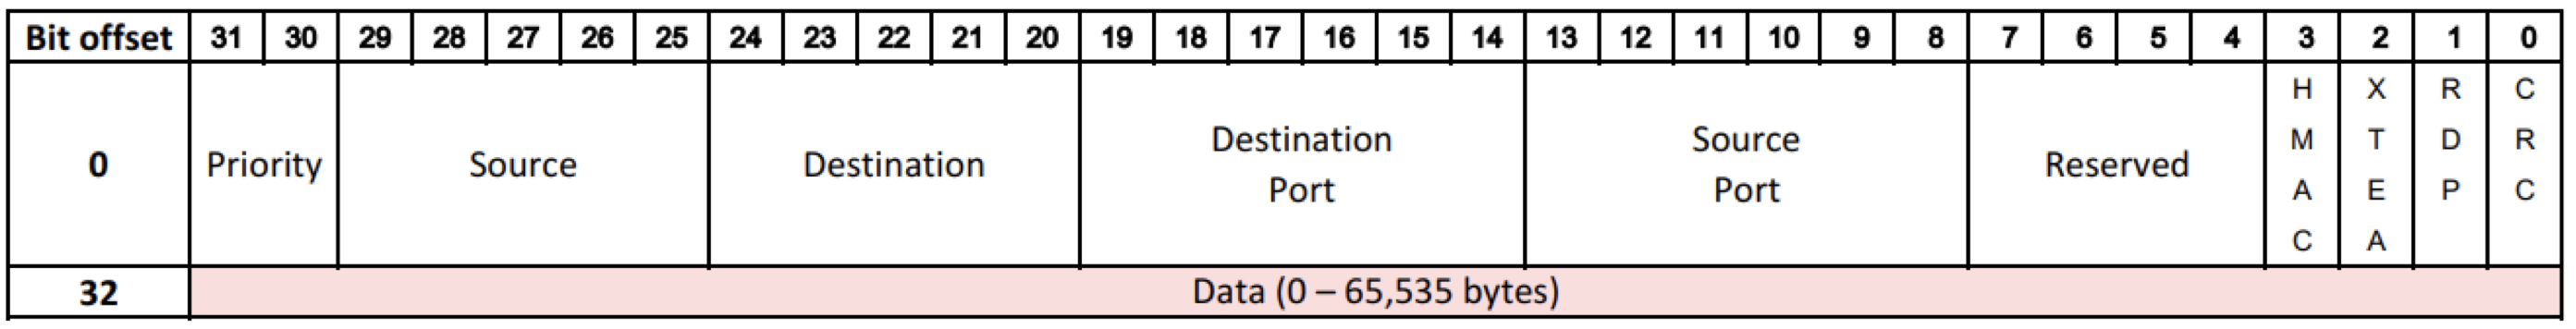
\includegraphics[width=\linewidth]{images/csp-header}}
    \caption{CSP header \cite{grillmayer}}
    \label{csp-header}
\end{figure}

The protocol allows defining up to 32 addresses. The common topology is that addresses 0-15 are used on the space segment, and the others are used in the ground system. It allows easy routing in the network.\cite{GomSpace}

CSP enables every subsystem to offer services at the same network level, eliminating the need for any master node. A service-oriented architecture offers various advantages over the conventional master/slave topology. Namely, authors of the protocol mention these advantages: services maintain a relationship that minimizes dependencies between subsystems; reduces single point of failure; logic is divided into services to promote reuse; beyond descriptions in the service contract, services hide logic from the outside world, etc. 

The implementation of the CSP is written in GNU C and can be compiled for FreeRTOS or Zephyr, which are real-time operating systems, or it can be compiled for Linux. Implementation is called Lib CSP.\cite{libcsp}

LibCSP incorporates two Transport Layer protocols: UDP (unreliable datagram protocol) and RDP (reliable datagram protocol). UDP operates as a datagram service, preserving data structures from entry to exit at the transport layer. The simplicity of UDP makes it practical for request/reply-based communication, especially in time-sensitive applications where dropped packets are preferable to delayed ones. However, UDP has limitations, particularly in larger file transfers, where automatic data acknowledgment becomes essential. The RDP protocol offers additional features, like a three-way handshake, flow control, retransmission, and extended acknowledgment. These features enhance reliability and performance, making RDP suitable for scenarios where a more robust and controlled data transfer protocol is required.

CSP supports connection-less or connection-oriented connections. To allocate a new connection, we can use one of the provided functions: client connection (csp\_connect), open server socket for listening (csp\_socket), or accept an incoming connection to the server (csp\_accept()).

There are also functions for sending and receiving CSP packets or pinging.

The last main feature is the routing table. Because the CSP is a network protocol, we can configure the routing table and enable routing if we want to route the packet to a different location.

Various interfaces can be used as a data link layer, such as AX.25 (KISS), CAN, I2C, etc. However, the maximum transfer unit is based on the selected interface. For instance, if you want to send larger packets over the CAN interface, which only allows a frame size of 8 bytes, then you have to use a custom implementation of fragmentation protocol in the data link layer. Specifically for CAN, a small protocol has already been written in the library.

\section{Bluetooth Low Energy}
Because we are supposed to establish the communication between the nRF52 chip and the Ground station (PC) over Bluetooth, we will now describe Bluetooth Low Energy (BLE). BLE is a standard that is supported on the nRF52.

Bluetooth standard is managed by a Bluetooth Special Interest Group (SIG). The most popular protocols nowadays are Bluetooth Classic and Bluetooth Low Energy. BLE targets markets where there is demand for low power rather than throughput. BLE sends short bursts of data. Typically, after the transmission, the radio goes to the sleep state.\cite{NovelBits}

We will be using BLE as a data link layer or interface. So, there is a need to first establish a BLE connection that already implements the whole OSI model - called BLE stack (fig. \ref{ble}). On top of that, we will run the CSP.

\begin{figure}[htbp]
    \centerline{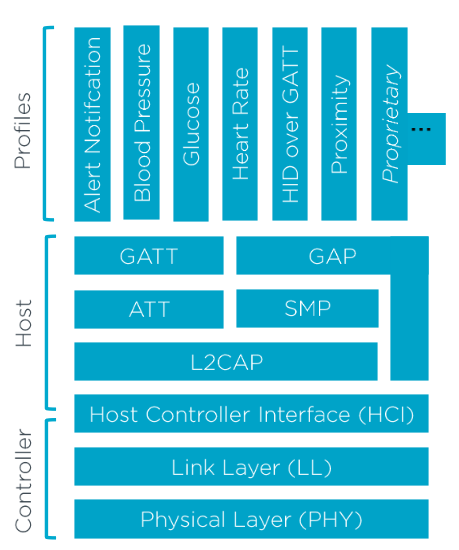
\includegraphics[width=\linewidth]{images/ble-stack}}
    \caption{Bluetooth Low Energy protocol stack \cite{ble-nordic-intro}}
    \label{ble}
\end{figure}

The architecture of the BLE stack can be divided into three subsystems - Controller, Host, and application.\cite{ble-nordic-intro}

The Controller contains a physical layer, which is a 2.4 GHz ISM band. It can use one of 40 RF channels (2 MHz per each) with GFSK modulation. The link layer defines the device address and manages the packet format.

The Host contains an Attribute Protocol (ATT). This layer provides a client-server model - the client device (typically phone/laptop) can access attributes on the server device (cubesat/IoT device). The SMP layer is the Security Manager Protocol, and it defines a protocol for pairing and key distribution if you want to use secured BLE.
Another layer that is already interesting from a developer's point of view is the GATT layer. GATT is the highest data layer and uses ATT to discover and access attributes. GATT defines the format of the data exposed by a BLE device. GATT specifies the structure of the attributes: services, characteristics, and descriptors.

Services are grouping one or more attributes. Service should satisfy a specific functionality on the server. Each service provides characteristics representing a piece of information the server wants to expose. An example of the service could be Heart Rate; it has characteristics like Heart Rate Measurement and Body Sensor Location.

The last layer from the Host component is GAP. The highest control layer defines how devices are discovered and connected (so-called advertisement). It also defines security modes.

On top of that, there are Profiles. Profile implements a specific application, and it can be standard or proprietary. Most of the time, the profiles are set by SIG. For instance, a standard Heart Rate Profile is used for medical and sports equipment. It consists of five standardized services: The Generic Access Service, Generic Attribute Service, Battery Service, Device Information Service, and Heart Rate Service. \cite{embeddedcentric}

\section{Laboratory part of the project}
Before you start, you must install a few dependencies: libsocketcan, cmake, git, and ninja-build.
\subsection{Modifications of libcsp}
We had to do some modifications of Lib CSP.

Having an interface with only two functions - write and read- is handy. The write function should be called on demand from libcsp and call Python's BLE send function. The read function should be called from the Python script when data over BLE is received. So, we modified the KISS interface, got rid of the UART driver, and provided only the mentioned functions in the new interface.
 
We created a new interface called Basic in lib cp/src/interfaces/csp\_if\_basic.h. The corresponding header file is in libcsp/include/csp/initerfaces/csp\_if\_basic.h. We also had to modify the CMake file in libcsp/src/initerfaces/CMakeLists.txt.
The news-provided interface contains these three functions:
\begin{enumerate}
    \item csp\_basic\_add\_interface - allocates and sets the new interface
    \item csp\_basic\_tx - called by libcsp when it needs to send data over BLE
    \item csp\_basic\_rx - called by Python to pass received packet to libcsp
\end{enumerate}

Unfortunately, while implementing these functions, we encountered a challenge where libcsp's attempt to invoke the tx function provided by Python resulted in a segmentation fault. The issue's root lay in Python's GIL (Global Interpreter Lock) and the fact that libcsp spawns new threads upon startup.

The GIL restricts the concurrent execution of Python bytecodes, hindering multi-core performance for CPU-bound tasks. While it maintains thread safety, the GIL necessitates workarounds, such as employing multiple processes or external libraries, to achieve true parallelism \cite{gil}.

This meant that libcsp's invocation of the tx function from a different thread triggered a segmentation fault. To overcome the GIL limitation and facilitate inter-process communication between libcsp and the Python script, we opted for ZeroMQ (Zero Message Queue). ZeroMQ is an asynchronous messaging library renowned for its high performance and ability to handle high-throughput data transfers. It provides a versatile set of sockets that enable various messaging patterns, such as publish-subscribe and request-reply, making it a powerful tool for building scalable and efficient distributed systems \cite{zmq}.

Now, when libcsp calls a tx function, the data packet is redirected to the python binding function (located in libcsp/src/bindings/python/pycsp.c) fnc\_tx that sends the packet over the ZeroMQ socket—the python script then retrieves the packet from the ZeroMQ socket and sends it over BLE interface.

We also implement Python binding functions to interact with the new basic interface. Namely
\begin{itemize}
    \item pycsp\_basic\_init - adding new basic interface and setting up ZeroMQ socket,
    \item pycsp\_basic\_rx - binding for calling csp\_basic\_rx.
\end{itemize}
These functions are located in libcsp/src/bindings/python/pycsp.c.

\subsection{nRF workspace installation procedure}
We are using nRF52832 DK as the development board. There are two available SDKs for this chip - nRF5 SDK, which is in maintenance mode and is not recommended to use it \cite{sdk}. The second SDK is called nRF Connect SDK \cite{connect}, used in this project. It is based on Zephyr. It is a real-time operating system. The main advantage of using real-time OS is that it allows us to create threads, although we use a single-core processor. It takes care of scheduling the threads. Fortunately, Zephyr is also an OS that Lib CSP natively supports.

To use nRF Connect SDK, follow instructions from nRF Connect SDK docs.

You need to install nRF Connect SDK extensions into your Visual Studio Code. Using a new profile in the VS Code; otherwise, the standard extensions for developing C projects will conflict.

Then, open the installed extension; from there, you can download Toolchain. After that, you should also download the SDK.

Now, it is time to include the Cubesat Space Protocol. Download the libcsp library. Now, you should navigate to the NCS folder where the SDK has been downloaded (under Linux, it should be in your home directory). Copy the libcsp library to the \lstinline{ncs/<sdk-version>/modules/lib} folder. Then you need to change \lstinline{ncs/<sdk-version>/nrf/west.yml}, so open it and find the line with the comment "Other third-party repositories." Under it, add the following two lines:
\begin{verbatim}
- name: libcsp
path: modules/lib/libcsp
\end{verbatim}

Then open folder nrf\_cubesat from the VS Code. Now, you need to create a new build. You need to choose the nrf52832dk\_nrf52832 profile. After that, you can build the project and flash the code.

\subsection{nRF project}
In this project, we are using an unsecured connection. For the communication, we are using Nordic UART Service (NUS). It is a proprietary GATT service that allows us to send byte arrays asynchronously. We chose this service because SIG defines no alternative. Implementation of NUS is already in the SDK. So, it only requires correctly setting up the BLE, and we don't have to do any low-level programming. In this service, there are two characteristics: Rx and Tx. The main issue with this UART emulation over BLE is that we can only send up to 20 bytes.

Two essential functions are in the main file. The first of them is ble\_write\_thread, which periodically sends data over BLE. Each 5 seconds, it sends a Hello World message with an incrementing integer.

A second important function is bt\_receive\_cb, which is called when data is received over BLE. Received data are printed into a log, and if received data is "1," it turns on LED3; if received data is "0," it turns off LED3.

\subsection{Ground station workspace - installation procedure}
The project for the "Ground Station" is located in folder pc\_cubesat. First, you must install a Python package called Bleak, which controls Bluetooth Low Energy. You can use the provided requirements.txt file or run: pip3 install bleak.

\subsection{Ground station project}
In the project, there are three Python files. The first file example\_ble\_uart.py, is compatible with nRF firmware, which has been described above. It prints what nRF sends over NUS (Nordic UART Service) and periodically sends 1 or 0 to toggle the LED3 on the DK board.

The second file, example\_csp\_server\_client.py, is an example file from the libcsp library. If you followed the installation procedure, you should be able to run it. When the address is set to 0, it probably uses a loopback interface.

The third file, csp\_python\_binding.py, is a script for testing a new interface called Basic, which we created. This script spawns a client task for CSP protocol and asynchronously handles the Basic interface and BLE connection. The asynchronous basic\_iface function contains an infinite loop that waits for data from the ZeroMQ socket. When the data packet is retrieved, it is sent to BLE. Also, when a new packet arrives from the BLE, the rx\_handler function is automatically called, and the packet is redirected into the CSP Basic interface through the pycsp\_basic\_rx function.

The current struggle is with the CSP library not responding to received packets. When calling the ping command from the client thread, the CSP library automatically calls TX functions, and data packets are sent through BLE. The packets are then successfully received on the second device and redirected to the CSP rx function. Unfortunately, this function is not provoking any response in the CSP library. The problem might lie in the CSP library itself or some network configuration error.

\newpage
\section{Conclusion}
In this report, we described the abstract OSI reference communication model. After that, we described Cubesat Space Protocol and Bluetooth Low Energy. These protocols are used in our lab project. 

Using emulated UART over BLE, we established communication between nRF DK and the Ground Station (PC). nRF runs on Zephyr, and Ground Station decodes packets received over BLE using the Python script. We also learned how to compile the CSP library on Zephyr - it is a few simple steps, but these steps needed to be better documented. We can also call Lib CSP functions from Python because we set up bindings between Python and Lib CSP. Last but not least, we provided a new simple interface called Basic, which can be used for direct data transfer between Lib CSP and our application.

We could not establish full automatic BLE communication with CSP protocol due to the library not responding to received packets. The possible solution might be the CSP network configuration or the library itself. Unfortunately, both are not well documented. 

\section*{Acknowledgment}
We want to thank the Space Engineering course team for lending us the hardware needed to create the work described here and for their advice on how to get started.

\bibliographystyle{unsrt}
\bibliography{bibliography}

\end{document}

